
\newtheorem{definition}{Definition.}


This chapter describes the \cgal's package for the extraction of
ridges and umbilics on meshes.  Given a smooth surface, a ridge is a
curve along which one of the principal curvatures has an extremum
along its curvature line. An umbilic is a point at which both
principal curvatures are equal. Umbilics are special points on the
ridge lines. Ridges are curves of {\em extremal} curvature and
therefore encode important informations used in segmentation,
registration, matching and surface analysis.  Based on the results of
the article
\cite{rr}, we propose several algorithms to identify and extract
different parts of this singular ridge curve as well as umbilics on a
surface given as a triangular mesh.


\subsection{Overview}
%%%%%%%%%%%%%%%%%%%%%%

2 main independent classes

\begin{itemize}
\item
\ccc{Umbilic_approximation}
\item
\ccc{Ridge_approximation}
\end{itemize}

And two ``container'' classes.

%%%%%%%%%%%%%%%%%%%%%%%
\section{Introduction}
\label{sec:intro}
%%%%%%%%%%%%%%%%%%%%%%%

\subsection{Ridges and umbilics of a smooth surface}
%%%%%%%%%%%%%%%%%%%%%%%%%%%%%%%%%%%%%%%

A comprehensive description of ridges can be found in
\cite{hgyg-ttdpf-99,ip-gd-01}, and in the sequel, we just
introduce the basic notions so as to explain our algorithms.
Consider a smooth embedded surface, and denote $k_1$ and $k_2$ the
principal curvatures, with $k_1\geq k_2$. Umbilics are the points
where $k_1=k_2$.  For any non umbilical point, the corresponding
principal directions of curvature are well defined, and we denote them
$d_1$ and $d_2$. 
%%
Anything related to the maximal (minimal) curvature is qualified blue
(red), for example we shall speak of the blue curvature for $k_1$ or
the red direction for $d_2$.
%%
In local coordinates, we denote $\langle , \rangle$
the inner product induced by the ambient Euclidean space, and $dk_1$,
$dk_2$ the gradients of the principal curvatures. Ridges, illustrated
on Figs \ref{pict:ellipsoid_ridges} and \ref{fig:ridges_ellipsoid},
are defined by:
%%
\begin{definition}
\label{def:ridge-extrema}
A non umbilical point is called
\begin{itemize}
\item
%a blue ridge point if $\langle dk_1,d_1 \rangle=0$,
a blue ridge point if the {\em extremality coefficient} $b_0=\langle
dk_1,d_1 \rangle$ vanishes, i.e. $b_0=0$.

\item
%a red ridge point if $\langle dk_2,d_2 \rangle=0$.
a red ridge point if the {\em extremality coefficient} $b_3=\langle
dk_2,d_2 \rangle$ vanishes, i.e. $b_3=0$.

\end{itemize}
\end{definition}
%We denote $b_0=\langle dk_1,d_1 \rangle$ and $b_3=\langle dk_2,d_2
%\rangle$, and we call these functions the {\em extremality
%coefficients}. 
%%
The previous characterization of ridges involves third-order
differential properties. Using fourth-order differential quantities, a
ridge point can further be qualified as {\em elliptic} if it
corresponds to a maximum of $k_1$ or a minimum of $k_2$, or {\em
hyperbolic} otherwise. Hence we end with four types of ridges, namely
: \ccc{BLUE_ELLIPTIC_RIDGE}, \ccc{BLUE_HYPERBOLIC_RIDGE}, \ccc{RED_ELLIPTIC_RIDGE},
\ccc{RED_HYPERBOLIC_RIDGE}.
In addition, a subset of elliptic ridges, called the crest lines,
which can be seen as the visually most salient curves on a surface are
also of interest. A crest line is an elliptic ridge which is a maximum
of $\max(|k_1|,|k_2|)$. Hence we provide two additional ridge types :
\ccc{BLUE_CREST} and \ccc{RED_CREST}.

Weigths are associated to each line
\begin{itemize}
\item
the {\bf strength} which is the integral of the curvature along the
line.
\item
the {\bf sharpness} which is the integral of the absolute value of
the second derivative of the curvature along the ridge.
\end{itemize}

%\begin{minipage}[c]{.45\linewidth}

\begin{figure}[!ht] 
\begin{ccTexOnly}
\centerline{ 
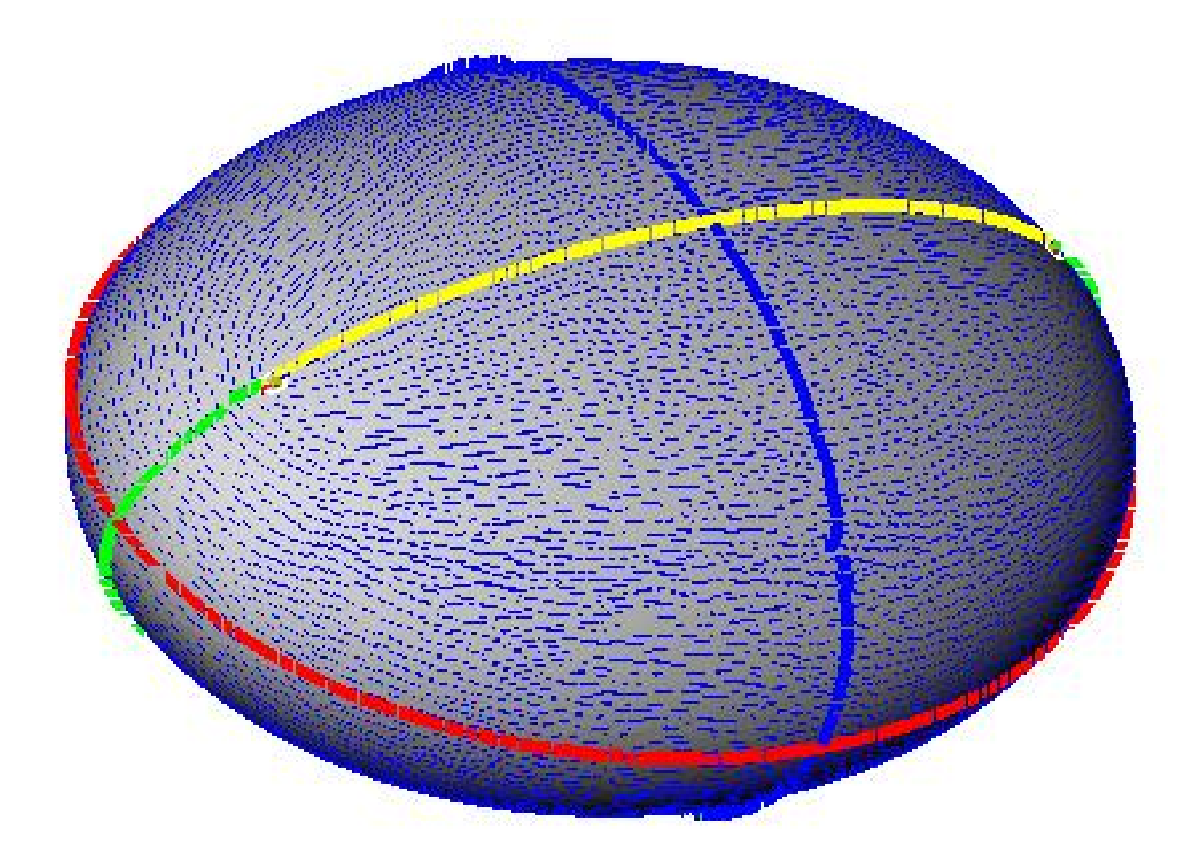
\includegraphics[height=5cm]{Ridges_3/ellipsoid_ridges_mesh}}
\end{ccTexOnly}

\begin{ccHtmlOnly}
<CENTER> <img border=0 src="./ellipsoid_ridges_mesh.jpg" width=400>
</CENTER>
\end{ccHtmlOnly}

\caption{Umbilics, ridges, and principal blue foliation on the
ellipsoid (10k points)}
\label{pict:ellipsoid_ridges} 
\end{figure} 
%\end{minipage}
%%
\hfill
%%
%\begin{minipage}[c]{.45\linewidth}
\begin{figure}[H] 
\begin{ccTexOnly}
\centerline{ 
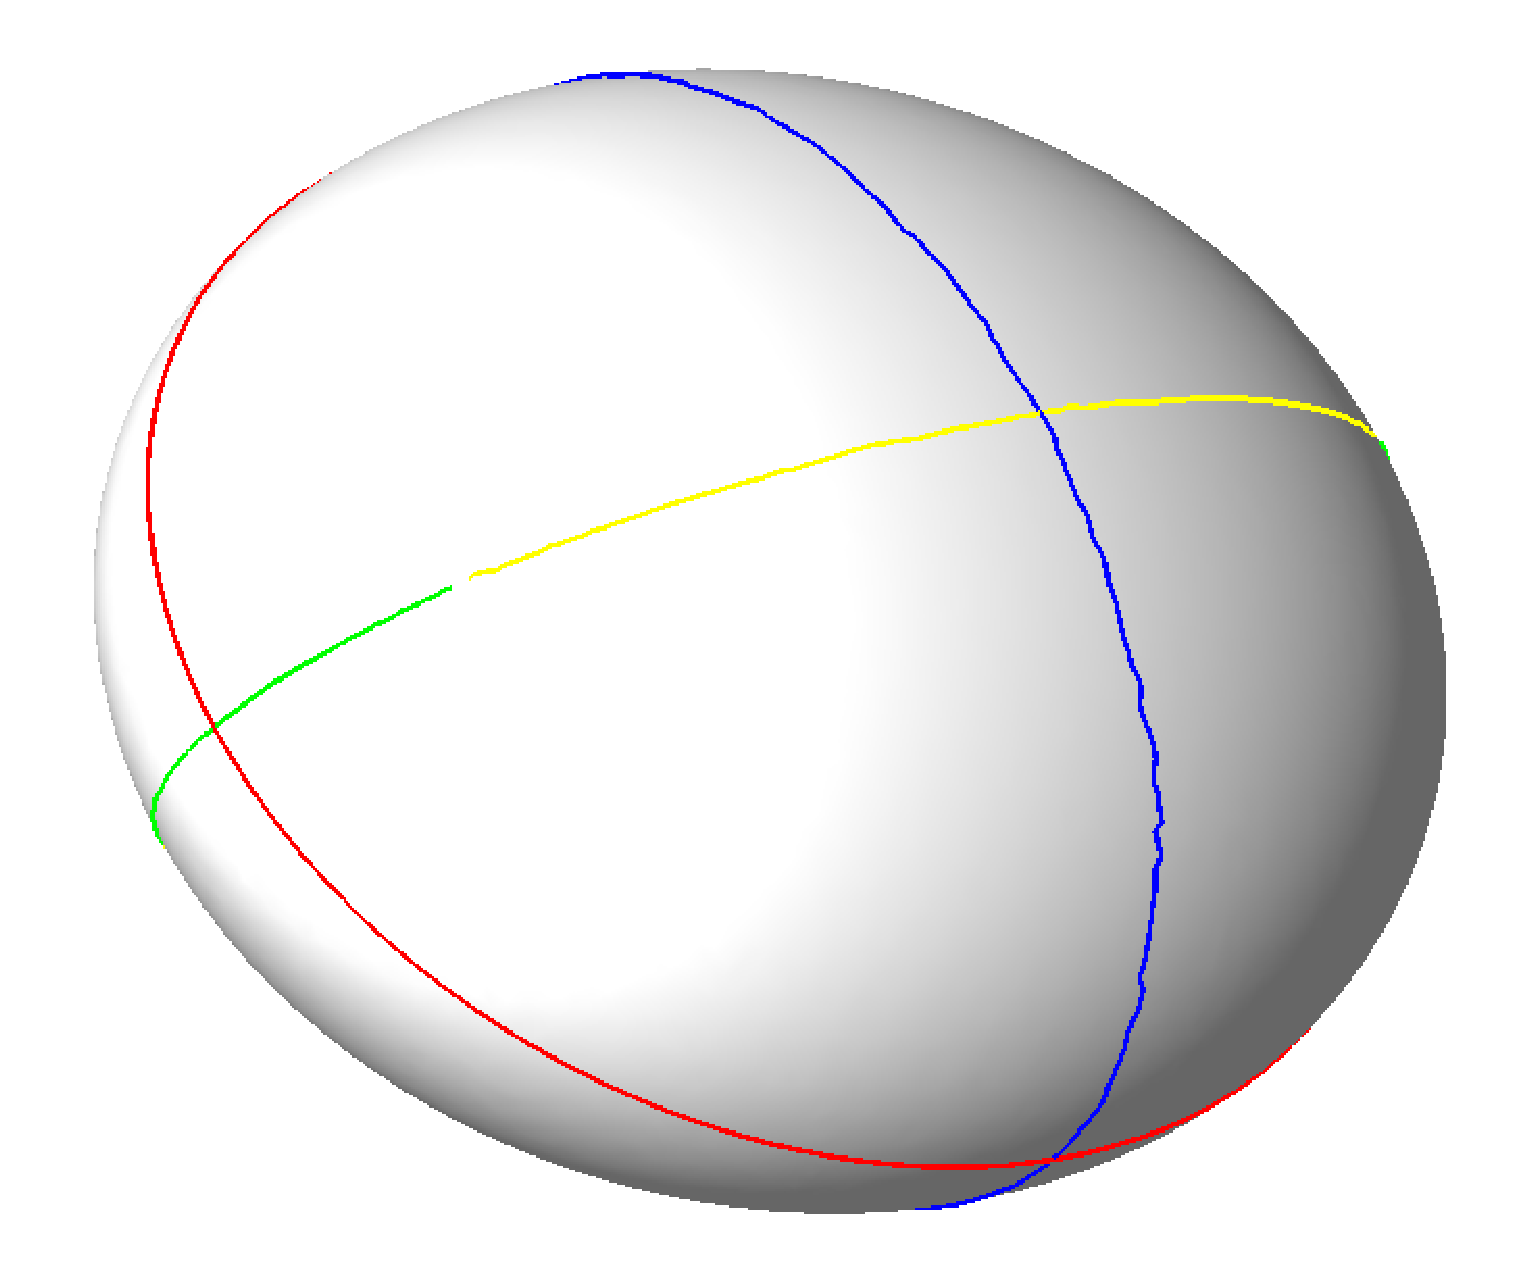
\includegraphics[height=5cm]{Ridges_3/ellipsoid_ridges}}
\end{ccTexOnly}

\begin{ccHtmlOnly}
<CENTER> <img border=0 src="./ellipsoid_ridges.jpg" width=400>
</CENTER>
\end{ccHtmlOnly}

\caption{Schematic view of the umbilics and the ridges. Max of $k_1$:
blue; Min of $k_1$: green; Min of $k_2$: red; Max of $k_2$: yellow}
\label{fig:ridges_ellipsoid}
\end{figure} 
%\end{minipage}



%%%%%%%%%%%%%%%%%%%%%%%
\section{Software Design}
%%%%%%%%%%%%%%%%%%%%%%%

usage of pm, triangular meshes.

\subsection{Options and interface specifications}
%%%%%%%%%%%%%%%%%%%%%
ridges: approx and container class

ridges compute with para type and tag

Umbilics : approx and container, 

umbilic compute with para 
size

\subsection{Template parameters}
%%%%%%%%%%%%%%%%%%%%%%%%%%%%%%%%%

On a des concepts: Vertex2FTPropertyMap et Vertex2VectorPropertyMap
qui sont specialisent le concept de Propety Map de boost, avec
\ccc{key_type CGAL::Polyhedron_3::Vertex_handle} et de \ccc{value_type
CGAL::Polyhedron_3::Traits::FT ou Vector_3 }. On a donc les fct get,
put, []; preciser LvaluePropertyMap ? Utilisation stockage
d'information scalaire ou vectorielle pour les vertex d'un polyhedron,
peut-etre dans le vertex lui-meme ou externe avec une std::map par
exemple. 

Poly est un concept qui a pour model \ccc{CGAL::Polyhedron_3} (faut-il
detaille les requirements?) TriangularPolyhedralSurface?

OutputIt est un concept de stl Output Iterator avec \ccc{value_type
CGAL::Ridge_line*} .\\
ou Outputit est un Output Iterator de la stl sur des Umbilic*


\subsection{Output}
%%%%%%%%%%%%%%%%%%%%

Classes \ccc{Umbilic} and \ccc{Ridge_line}

%%%%%%%%%%%%%%%%%%%%%%%%%%%%%%%%%%%%%%%%%%%%%%%%%%%%%%%%%%%%%%%%%%%%%%%%%%%%
\section{Examples} 
%%%%%%%%%%%%%%%%%%%%%%%%%%%%%%%%%%%%%%%%%%%%%%%%%%%%%%%%%%%%%%%%%%%%%%%%%%%%
